\documentclass{article}
\usepackage[utf8]{inputenc}
\usepackage[T1]{fontenc}
\usepackage{minted}
\usepackage{graphicx}
\usepackage{float}
\usepackage{onecolceurws}
\usepackage{hyperref}
\usepackage{lmodern}
\hypersetup{
    colorlinks=true,
    linkcolor=blue,
    filecolor=magenta,      
    urlcolor=cyan,
}
\urlstyle{same}
\title{ A Survey on Leveraging Entities in Ad-Hoc Document Retrieval}

\author{
Shubham Chatterjee \\ sc1242@cs.unh.edu
}
\institution{Department of Computer Science, University of New Hampshire, Durham NH 03824, USA}

\begin{document}

\maketitle

\begin{abstract}
With the huge amount of unstructured data in the form of text at our disposal, being able to efficiently search and retrieve information from this data is an important problem. The field of Information Retrieval (IR) is concerned with developing technology for matching \textit{information needs} with \textit{information objects}\cite{balog2018entity}. The information need may range from a few simple keywords to a natural language question whereas the information object has traditionally been passages or documents. However, as large-scale structured knowledge repositories (called \textit{knowledge bases}), which organize information around specific things or objects (called \textit{entities}) have become available, rich semantic information has become available which may help to improve the quality of the search results (passages or documents). In this paper, we present a brief survey of methods available in the literature for leveraging this semantic information (in the form of entities) for document retrieval.  


 %Analysis of web search query logs has shown that a large portion of the queries now contain some entity, reflecting an increase in the demands of users on retrieving relevant information about entities such as persons, organizations, products, etc. Advances in information extraction allow us to efficiently extract entities from free text. Since an entity is expected to capture the semantic content of documents and queries more accurately than a term, it would be interesting to study whether leveraging the information about entities can improve the retrieval accuracy. Moreover, several studies indicate that 40-70\% of all web searches target entities. In such cases, it is pertinent to explain to the user how the retrieved entity is related to the original query. With an increase in the focus on entities for search, it becomes necessary to organize them in a structure which is suitable for efficient retrieval. Knowledge Graphs provide a way to structure semantic information which can be used effectively in search. Such knowledge graphs contain entities as nodes with the relationships between them as edges. Explaining such entity relationships is another common information retrieval task. In this paper, we present a brief survey of methods available in the literature for leveraging entities in search. 
\end{abstract}
\vskip 32pt

\section{Introduction}
\label{sec:introduction}

In the modern world, search engines are an integral part of human lives. We use Google, Bing, Baidu, etc. every moment as the main gateway to find information on the Web. %We search for people, organizations and events on Facebook and LinkedIn; for products on Amazon and eBay; or for music on YouTube or Spotify. 
With the smartphones becoming ubiquitous, we have increasingly come to depend on search functionality to find contacts, email, notes, calendar entries, apps, etc.  
The field of Information Retrieval (IR) is concerned with developing technology for matching \textit{information needs} with \textit{information objects}. According to Manning et al. \cite{Manning:2008:IIR:1394399}, 
\begin{quote}
    \textit{\textbf{Definition 1:}} Information Retrieval (IR) is finding material (usually documents) of an unstructured nature (usually text) that satisfies an information need from within large collections (usually stored on computers)
\end{quote}
Our query, i.e., the information need, may range from a few simple keywords (e.g., \textit{dark chocolate health benefits}) to a proper natural language question (e.g., \textit{Who are the members of Eagle?}). The search engine then displays a ranked list of results, i.e., information objects relevant to our query. Traditionally, these items were documents. In fact, IR has been seen as synonymous with document retrieval by many. Traditional document retrieval models such as  Term Frequency Inverse Document Frequency(TF-IDF) \cite{jones1988, salton1988term,robertson1976relevance,croft1979using,papineni2001inverse}, BM25 \cite{jones2000probabilistic} and Language Models \cite{ponte1998language} are term based models and do not have any notion of semantics in them. For example, TF-IDF is a statistical measure used to evaluate how important a word is to a document in a collection or corpus. The importance increases proportionally to the number of times a word appears in the document but is offset by the frequency of the word in the corpus, which helps to adjust for the fact that some words appear more frequently in general. Similary, BM25 is a \textit{bag-of-words}(text represented as the bag (multiset) of its words, disregarding grammar and even word order but keeping multiplicity) retrieval function that ranks a set of documents based on the query terms appearing in each document, regardless of their proximity within the document whereas Language Models are probability distributions over sequences of words where a separate language model is associated with each document in a collection and documents are ranked based on the probability of the query $Q$ in the document's language model $M_d$ ($P(Q \vert M_d)$. None of these models consider the semantic relationship between various places, events, orgaizations, etc. in the query or the document.

However, there has been a dramatic shift in paradigm in the last decade with the focus shifting to leveraging the rich semantic information available in the form of \textit{entities}. Analysis of web search query logs has shown that a large portion of the queries now contain some entity, reflecting an increase in the demands of users on retrieving relevant information about entities such as persons, organizations, products, etc. Advances in information extraction allow us to efficiently extract entities from free text. Since an entity is expected to capture the semantic content of documents and queries more accurately than a term, there has been much research in using entities to aid document retrieval and ranking. In this paper, we provide a brief overview of the existing methods in literature for leveraging entities for passage retrieval. We then describe our current work in progress on explaining query-entity relationships and then using these explanations to derive a better passage ranking. 

\section{Background}
\label{sec:background}
\subsection{What is an Entity?}
\label{subsec:what-is-an-entity}

Informally, we call an entity as a ``thing'' or ``object'' that one can refer to such as people, locations, products, organizations, and events. However, consider the entity \textit{Apple}. Does this refer to the fruit or the company? Identifying entities is an important and difficult task addressed by people in both the Natural Language Processing (NLP) as well as IR community (although traditionally, the task has been looked upon as more of a NLP problem than an IR problem). Balog \cite{balog2018entity} defines an entity as follows, taking inspiration from the Entity-Relationship (ER) Model proposed by Chen \cite{Chen:1976:EMU:320434.320440} in 1976:
\begin{quote}
    \textit{\textbf{Definition 2:}} An \textit{entity} is a uniquely identifiable object or thing, characterized by its name(s), type(s), attributes, and relationships to other entities.
\end{quote}
We restrict our universe to some particular registry of entities, which we will refer to as the \textit{entity catalog}. Thus, we consider that an entity ``exists'' if an only if it is an entry in the given entity catalog. Thus:
\begin{quote}
    \textit{\textbf{Definition 3:}} An \textit{entity catalog} is collection of entries, where each entry is identified by a unique ID and contains the name(s) of the corresponding entity.
\end{quote}

\subsection{Representing Entity Properties}
\label{subsec:representing-entity-properties}

Consider the Wikipedia page of Barrack Obama. It contains information about him ranging from his early life, education, early career in law to his rise to US Presidency. Hence, to us humans, Wikipedia is a \textit{Knowledge Repository}. According to Balog \cite{balog2018entity}:
\begin{quote}
    \textit{\textbf{Definition 4:}} A \textit{Knowledge Repository} (KR) is a catalog of entities that contains entity type information, and (optionally) descriptions or properties of entities, in a semi-structured or structured format.
\end{quote}
Wikipedia is a classic example of a knowledge repository. Each article in Wikipedia is an entry that describes a particular entity. Articles are also assigned to categories (which can be seen as entity types) and contain hyperlinks to other articles (thereby indicating the presence of a relationship between two entities, albeit not the type of the relationship). Wikipedia articles also contain information about attributes and relationships of entities, but not in a structured form.

With the development of knowledge repositories such as Wikipedia, a lot more information about entities have become available but for machines, this knowledge needs to be represented explicitly. A \textit{Knowledge Base}(KB) is comprised of a large set of assertions about the world. To reflect how humans organize information, these assertions describe (specific) entities and their relationships. An AI system can then solve complex tasks, such as participating in a natural language conversation, by exploiting the KB. According to Balog \cite{balog2018entity}:
\begin{quote}
    \textit{\textbf{Definition 5:}} A \textit{Knowledge Base} (KB) is a structured knowledge repository that contains a set of facts (assertions) about entities.
\end{quote}
Conceptually, entities in a knowledge base may be seen as nodes of a graph, with the relationships between them as (labeled) edges. Thus, especially when this graph nature is emphasized, a knowledge base may also be referred to as a \textit{Knowledge Graph} (KG).

%\textit{Outline.} The remainder of this paper is organized as follows.

%\begin{figure}[t]
% \centering 
 %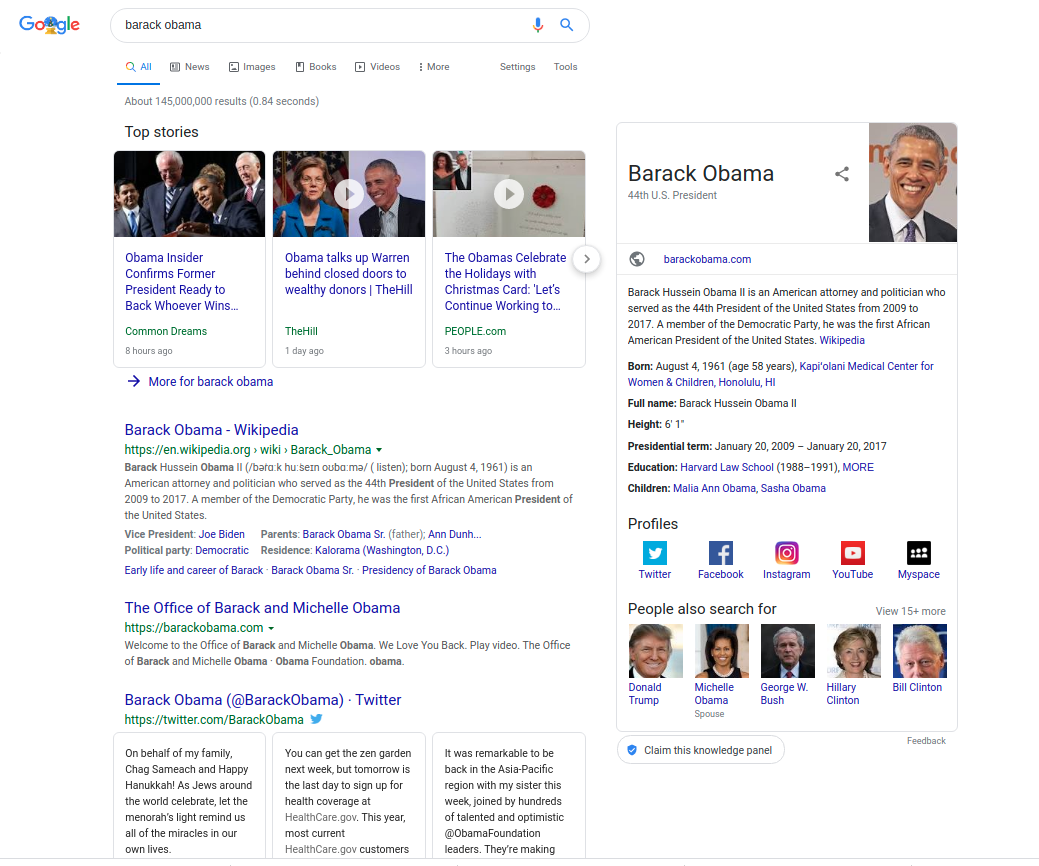
\includegraphics[scale=0.44]{entity-card.png}
 %\caption{Google search results for the query \textit{barrack obama} showing an \textit{entity card} on the right.}
% \label{fig:entity-card}
%\end{figure}

\section{Ad-Hoc Document Retrieval Using Entities}
\label{sec:doc-ret-using-ent}
The ``Ad-Hoc'' document retrieval task is defined as follows:

\textbf{Ad-Hoc Document Retrieval.} Given a query and a corpus, find the relevant documents.\\
The \textit{query} is a textual description of an information need such as \textit{Who is the president of the US?} or \textit{water pollution}. The \textit{corpus} is a collection of textual documents and \textit{relevance} is defined as the satisfaction of the user's information need. It is called \textit{Ad-Hoc} because the number of possible queries is huge. 

In this section, we review the work in which entities have been used for the ad-hoc document retrieval task.

\subsection{Entity Query Feature Expansion (Dalton et al.\cite{dalton2014entity})}
\label{subsec:eqfe}

The motivation behind Entity Query Feature Expansion (EQFE) is the fact that with advances in automatic entity linking and knowledge base construction, entity annotations for document and query collections have become available. These entity annotations could possibly be used in ad-hoc document retrieval. Towards that goal, the authors propose to extend the query with various features including entity name, entity links and attributes in knowledge base, entity context model, collection feedback, etc., as opposed to performing traditional query expansion on the text representation. The final query-document relevance is based on the integration of relevance between document and all the query features. EQFE uses enriched features to aggregate relevance between query and documents and requires learning-to-rank based parameter tuning to acquire parameters as the number of parameters is proportional to the number of features.It requires explicit entity annotation in relevant documents to improve the performance as some important features rely on such annotations.

\subsection{EsdRank (Xiong et al.\cite{xiong2015esdrank})}
\label{subsec:esdrank}

EsdRank uses external semi-structured data such as controlled vocabularies and knowledge bases and treats vocabularies, terms and entities from external data, as objects connecting query and documents. The evidence from the query, external data, and corpus is incorporated as features to express the relationship between query, object and document. A new ranking model called Latent-ListMLE (based on the learning to rank model called ListMLE) is used to rank documents with these objects and evidence. Like ListMLE, Latent-ListMLE too defines the probability of a ranking being generated by a query in a parametric model and uses Maximum
Likelihood Estimation (MLE) to find parameters that maximize the likelihood of the best ranking(s). Moreover, it assumes that the probability of a document being ranked at position $i$ is independent of those ranked at previous positions (due to the sample space of all possible rankings being too large). However, unlike ListMLE, Latent-ListMLE adds a latent layer in the ranking generation process. The latent layer contains related objects as possible representations of the original query. 

\subsection{Latent Entity Space (Liu et al.\cite{liu2015latent})}
\label{subsec:les}

Latent Entity Space (LES) uses entities to represent the semantic content of document and queries. The key idea is to construct a high-dimensional latent entity space, in which each dimension corresponds to one entity, and map both queries and documents to the latent space accordingly. The relevance between query and document is then estimated based on their projections to each dimension in the latent space. This is in contrast to the traditional term-based retrieval models, which estimate the query-document relevance in a high-dimensional term space. Each dimension is represented using the entity's profile. This profile is created in two ways: by pooling pieces of information from documents mentioning the entity and by using knowledge bases such as DBPedia. Only those entities which are most related to the query are used to create the LES. 

\subsection{Query Expansion with Freebase (Xiong et al.\cite{xiong2015query})}
\label{subsec:query expansion with freebase}

This paper focuses on using a knowledge base (Freebase) for the purpose of query expansion and ranks documents using the expanded query. Given a query, the task is to find relevant entities for the query and use the information about the entities to expand the original query and re-rank an initial candidate set of documents for the query

%Two tasks are identified:
%\begin{itemize}
%    \item \textbf{Entity Ranking}. Given a query,  find relevant entities for the query.
 %   \item \textbf{Document Ranking}. Use the information about the entities obtained above to expand the original query and re-rank an initial candidate set of documents for the query.
%\end{itemize}
They propose an unsupervised and a supervised method for expansion using Freebase. 
\begin{itemize}
    \item \textbf{Unsupervised Method}. This is done in two steps:
    \begin{itemize}
        \item \textit{Object Linking}. This is done by either retrieving objects directly from Freebase or selecting them from the annotations in top ranked documents for the query.
        \item \textit{Term Selection}. This is done by either using the \textit{tf-idf} information from the object's Freebase description or by using the similarity of query and the term’s distributions in Freebase’s categories. 
    \end{itemize}
    \item \textbf{Supervised Method}. A supervised model combines information derived from Freebase descriptions and categories to select terms that are effective for query expansion. The following three scores describing the relationship between a query-term pair are used as features:
    \begin{enumerate}
        \item \textit{tf-idf} Pseudo Relevance Feedback score in retrieved objects.
        \item \textit{tf-idf} Pseudo Relevance Feedback score in top retrieved documents’ FACC1 \footnote{FACC1 is the Freebase annotation of TREC queries and ClueWeb corpora provided by Google} annotations.
        \item Negative Jensen-Shannon divergence score between category distributions.
    \end{enumerate}
    The three scores are used as features for a supervised model that learns how to select better expansion terms. All terms in linked objects’ descriptions are used as candidates for query expansion. The ground truth score for a candidate term is generated by its influence on retrieved documents, when used for expansion individually. If a term increases the ranking scores of relevant documents, or decreases the ranking scores of irrelevant documents, it is considered to be a good expansion term, and vice versa.
\end{itemize}
Once expansion terms are selected, the initial set of candidate documents retrieved for the query are re-ranked using a ranking model which is a weighted combination of the initial retrieval score of the document and the retrieval score of the term. 

\subsection{Entity-Based Language Models (Raviv et al.\cite{raviv2016document})}
\label{subsec:eblm}

The authors present various entity-based language models to address the task of ad-hoc document retrieval. Previous work have focused on either projection based methods \cite{liu2015latent} or expansion based methods \cite{xiong2015query}. This paper studies whether the markup of entities in a query and documents is, by itself, sufficient information for improving retrieval effectiveness. Various entity-based language models which consider both single terms in the text as well as term sequences marked as entities by an existing entity-linking tool, are proposed. These language models are induced from the query and documents in the corpus and serve for retrieval in the language modeling framework. The main novelty of these language models is accounting, simultaneously, for (i) the
uncertainty in entity linking — specifically, the confidence levels of entity markups; and, (ii) the balance between using term-based and entity-based information. A document is ranked by the cross entropy between the language models induced from the query and the document.

\subsection{Bag-of-Entities Representation for Ranking (Xiong et al. \cite{xiong2016bag})}
\label{subsec:bag of entities}

Bag-of-Words is a common technique of representing queries and documents in IR. This paper describes a Bag-of-Entities representation for query and documents and evaluates its performance on a publicly available dataset. They use 3 entity linking systems to annotate query and documents with Freebase entities. These are \textit{FACC1}, \textit{TagMe} and \textit{CMNS}\footnote{CMNS is an entity linking system that spots texts using surface forms from FACC1 annotation, and links all of them to their most frequently linked entities}.
%\begin{itemize}
%    \item \textbf{FACC1}.
%    \item \textbf{TagMe}.
%    \item \textbf{CMNS}. It is an entity linking system that spots texts using surface forms from FACC1 annotation, and links all of them to their most frequently linked entities
%\end{itemize}
Bag-of-Entities vector for the query and documents are created using the entity annotations and two ranking models are used to re-rank an initial candidate set of documents for the query. The first model called ranks a document by the number of query entities it contains and the second ranks a document by the frequency of query entities in it.

\subsection{Semantic Enabled Language Model (Ensan et al.\cite{ensan2017document})}
\label{subsec:selm}

Semantic Enabled Language Model (SELM) addresses the task of document retrieval based on the degree of document relatedness to the meaning of a query. It is based on using an entity linking system to extract concepts (entities) from documents and queries. The document is represented as a graph where the nodes are the concepts and the edges are the relatedness relationship between two concepts. The documents are ranked by finding the conditional probability of generating the concepts observed in the query given all the document concepts and the relatedness relationships between them. Hence, SELM (as the name suggests) is a language model which given the semantic relatedness between the observed concepts, finds the probability that a query concept is generated from a specific document, much on the lines of traditional IR language models.

\subsection{JointSem (Xiong et al.\cite{xiong2017jointsem})}
\label{subsec:jointsem}

JointSem presents a joint semantic ranking method that combines query entity linking and entity-based document ranking. A dictionary containing mappings from surface forms of entities to candidate entities in constructed. This dictionary contains all possible surface forms of entities and is collected from Wikipedia. JointSem consists of the follwing three steps:
\begin{enumerate}
    \item \textbf{Spotting}. N-grams in the query are looked up in the surface form dictionary. Start from the first word, spot the longest surface forms, and move to the word after the surface form. No overlapped spots are allowed. Several features are extracted to describe the reliability of the surface form.
    \item \textbf{Linking}. In this step, the spotted surface forms are aligned with candidate entities. If a surface form has several candidate entities, the authors link all of them to avoid over-committing. Several features are extracted to describe the relevance of the entity to the query.
    \item \textbf{Ranking}. The entity’s name and description and the document’s title and body are used to extract several entity-document features using standard IR models such as BM25, Language Models with Dirichlet Smoothing, TF-IDF and Coordinate Match. These features are used to rank the documents for the query. The ranking model consists of three parts: The first part learns the importance of the surface form, the second part learns the importance of the aligned entity and the third part learns the ranking of document for the entity. The three parts are combined for the final ranking score and trained using standard pairwise learning-to-rank with hinge loss by standard back-propagation.
\end{enumerate}

\subsection{Explicit Semantic Ranking (Xiong et al.\cite{xiong2017explicit})}
\label{subsec:esr}

\subsection{Word-Entity Duet Representations for Document Ranking (Xiong et al.\cite{xiong2017word})}
\label{subsec:word entity duet}

\subsection{Kernel Entity Salience Model (Xiong et al.\cite{xiong2018towards})}
\label{subsec:kesm}






\bibliographystyle{acm}
\bibliography{references}
\end{document}
